\documentclass[12pt,a4paper]{article}
% \usepackage[portuges]{babel}
% \usepackage[utf8]{inputenc}
% \usepackage[T1]{fontenc}
\usepackage{hyperref}
\usepackage{url}
\usepackage{graphicx}
\usepackage{float}
\usepackage{enumerate}
\usepackage{makeidx}
\usepackage{booktabs}
\usepackage{longtable}
\usepackage{pdfpages}
\usepackage{a4wide}
\usepackage{xcolor}

\setlength\oddsidemargin{0.3in}
\setlength\evensidemargin{-0.3in}
\setlength\headsep{15pt}
\setlength\footskip{30pt}

\usepackage{fontspec}
\defaultfontfeatures{Mapping=tex-text}
\setmainfont[
  Extension=.ttf,
  Path=font/,
  Scale=1.00,
  BoldFont={NewsGotTMed Regular},
  ItalicFont={NewsGoth Lt BT Light},
  ItalicFeatures={FakeSlant},
  AutoFakeSlant=0.3,
  BoldItalicFeatures=FakeSlant, 
]{NewsGotT Regular Fixed}

%Line Spacing
\usepackage{xspace}
\usepackage{setspace}
\onehalfspacing

% Language definitions
\usepackage{polyglossia}
\setmainlanguage{portuges}



% environment created for organization purposes, only.
\newenvironment{TODO}{%
  \color{blue} \itshape \begin{itemize}
}{%
  \end{itemize}
}

%---------------------------------------

% our addimage command
\newcommand{\addimg}[1]{%
  \begin{center}
    \includegraphics[width=0.75\textwidth]{#1}
  \end{center}
}

\newcommand{\RowStretch}[1]{\renewcommand{\arraystretch}{#1}}


%----------------------------------------------------------

\begin{document}

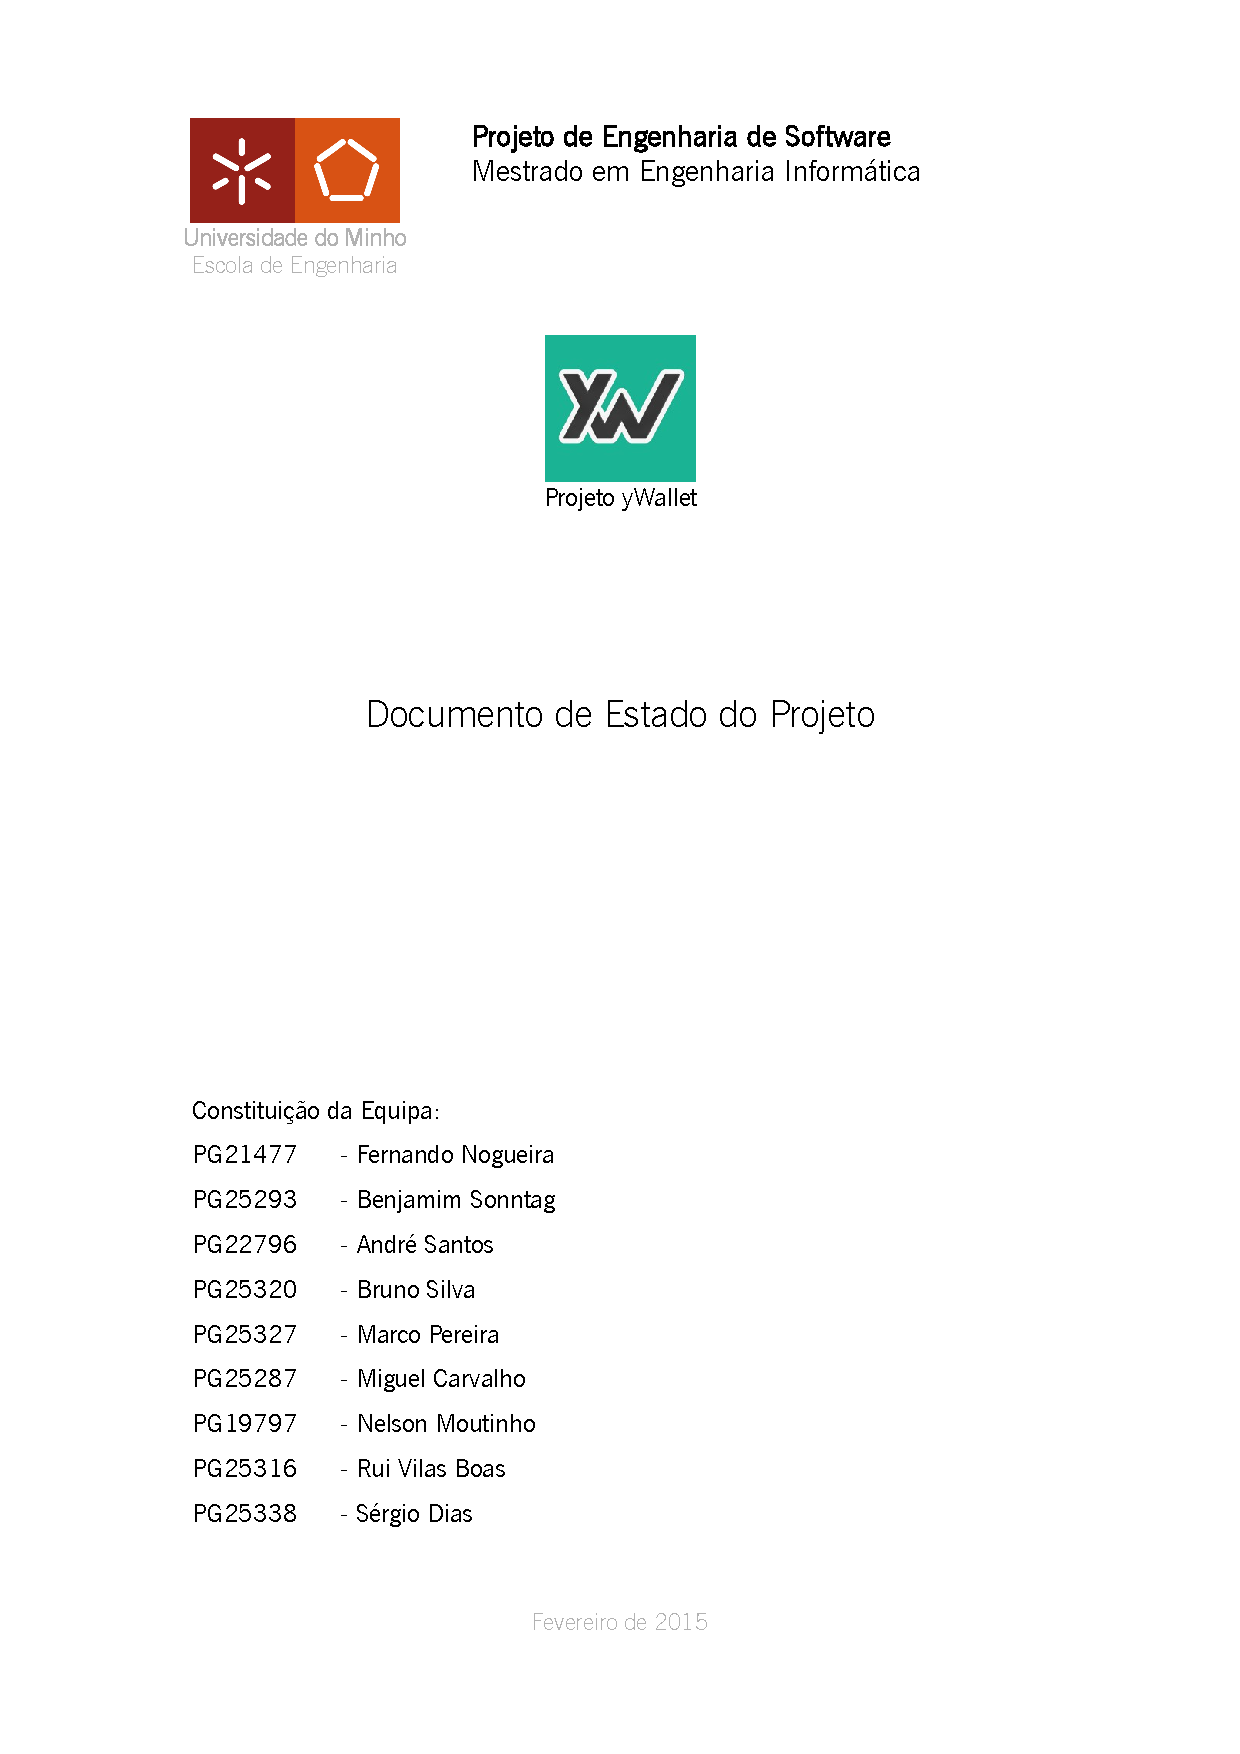
\includepdf[pages=-]{capa}

\section*{Estado do Projeto}
\label{sec:state}
O presente documento relata e resume o estado atual do projeto, em relação às funcionalidades presentes, funcionalidades pendentes, e os requisitos impostos.

Na Tabela \ref{tab:func} são apresentadas as funcionalidades ou requisitos funcionais planeados na fase inicial deste projecto, e é indicado, para cada uma deles, se foram implementados com sucesso. A Tabela \ref{tab:non_func} apresenta o mesmo sumário para os requisitos não-funcionais.

De um modo geral, os requisitos mais importantes foram satisfeitos, pelo menos parcialmente. As principais falhas, em funcionalidades parcialmente implementadas, devem-se a ajustes em falta na comunicação entre cliente e servidor, falta de suporte para a operação por parte do servidor, ou interfaces incompletas na aplicação.
Algumas funcionalidades sofreram ajustes na sua priorização inicial, de modo a que a equipa se pudesse adaptar melhor aos prazos a cumprir. A geolocalização é um exemplo das funcionalidades que foi deixada para trabalho futuro. A priorização inicial de cada requisito está também presente nas tabelas abaixo, segundo o esquema MoSCoW.

Resumindo, este projeto ainda se encontra numa fase de desenvolvimento ativo, para que possa oferecer um mínimo satisfatório de funcionalidades aos seus utilizadores. O foco atual do desenvolvimento encontra-se em simplificar a comunicação entre a aplicação e o servidor, concretizar as transferências monetárias, e mostrar ao utilizador toda a informação que este deve ser capaz de consultar. Daí em diante, o foco incidirá no suporte ao utilizador no uso e aprendizagem da aplicação. Por fim, todos os requisitos não-funcionais serão revisitados e satisfeitos no produto final.

\begin{center}
    \RowStretch{1.2}
\begin{longtable}{@{}lcp{0.3\textwidth}cp{0.3\textwidth}@{}}
    \toprule \#  & MoSCoW & Funcionalidade    & Estado   & Observações \\ \midrule
    \endfirsthead
    \toprule \#  & MoSCoW & Funcionalidade    & Estado   & Observações \\ \midrule
    \endhead
    \bottomrule
    \caption{Sumário dos requisitos funcionais.}\label{tab:func}\\%
    \endfoot
    \bottomrule
    \caption[]{Sumário dos requisitos funcionais.}\\%
    \endlastfoot
    \multicolumn{5}{l}{\color{gray} Uso Geral da Plataforma} \\
    1   & M & Criar conta de utilizador. & Concluído  &  \\
    2   & M & Editar informação de utilizador. & Concluído  &  \\
    3   & M & Associar conta de serviço de gestão de dinheiro. & Concluído  &  \\
    \multicolumn{5}{l}{\color{gray} Restrições de Uso de Dinheiro} \\
    4   & M & Definir limites de utilização do dinheiro em ordem ao tempo. & Parcial &  \\
    5   & C & Definir limites de utilização do dinheiro em ordem à localização. & A Fazer & A geolocalização foi deixada para trabalho futuro. \\
    \multicolumn{5}{l}{\color{gray} Consulta de Informação} \\
    6   & M & Consultar histórico de gastos. & Parcial  &  \\
    7   & M & Filtrar histórico de gastos por data. & Parcial  &  \\
    8   & C & Filtrar histórico de gastos por localização. & A Fazer & A geolocalização foi deixada para trabalho futuro. \\
    9   & M & Consultar estado de conta. & Parcial & Faltam acertos de comunicação entre cliente e servidor. \\
    \multicolumn{5}{l}{\color{gray} Notificações} \\
    10  & S & Definir regras de notificação simples. & Parcial &  \\
    11  & S & Definir regras de notificação complexas. & A Fazer & Um motor de regras de notificação flexível foi deixado para trabalho futuro. \\
    \multicolumn{5}{l}{\color{gray} Transferência de Dinheiro} \\
    12  & S & Autorizar o acesso a quantias de dinheiro extraordinárias, sem pedidos. & A Fazer &  \\
    13  & S & Receber e responder a pedidos de acesso a quantias de dinheiro. & Parcial & Falta suporte do servidor. \\
    14  & S & Efetuar pedidos de acesso a quantias de dinheiro. & A Fazer &  \\
    \multicolumn{5}{l}{\color{gray} Organização de Informação} \\
    15  & M & Gerar estatísticas do uso da conta. & A Fazer &  \\
    \multicolumn{5}{l}{\color{gray} Outros} \\
    16  & M & Efetuar pagamentos a comerciantes. & A Fazer &  \\
    17  & C & Transferir dinheiro para outros utilizadores. & A Fazer &  \\
    18  & C & Definir metas de poupança. & Parcial & Faltam acertos de comunicação entre cliente e servidor.
\end{longtable}
\end{center}

\begin{center}
    \RowStretch{1.2}
\begin{longtable}{@{}lcp{0.3\textwidth}cp{0.3\textwidth}@{}}
    \toprule \#  & MoSCoW & Requisito    & Estado   & Observações \\ \midrule
    \endfirsthead
    \toprule \#  & MoSCoW & Requisito    & Estado   & Observações \\ \midrule
    \endhead
    \bottomrule
    \caption{Sumário dos requisitos não-funcionais.}\label{tab:non_func}\\%
    \endfoot
    \bottomrule
    \caption[]{Sumário dos requisitos não-funcionais.}\\%
    \endlastfoot
    \multicolumn{5}{l}{\color{gray} Aparência} \\
    1   & S & Tema visual apelativo. & Concluído &  \\
    2   & M & Aspeto profissional, que transmita confiança. & Parcial &  \\
    \multicolumn{5}{l}{\color{gray} Usabilidade} \\
    3   & S & Produto fácil de aprender e utilizar. & Parcial &  \\
    4   & C & Produto multilingue. & Parcial &  \\
    5   & W & Aceitar várias moedas. & A Fazer &  \\
    6   & S & Usar uma linguagem simples e clara, de fácil entendimento. & Parcial  &  \\
    \multicolumn{5}{l}{\color{gray} Desempenho} \\
    7   & M & Não exceder os 5 segundos em carregamentos de dados. & Parcial  &  \\
    8   & M & Fluidez e bom desempenho nos dispositivos móveis. & Parcial &  \\
    9   & W & Disponibilidade de 99\% de um ano. & A Fazer &  \\
    10  & S & Precisão de valores monetários até à unidade transacional mais pequena. & Parcial &  \\
    11  & C & Recuperação rápida em resposta a falhas. & A Fazer &  \\
    \multicolumn{5}{l}{\color{gray} Operação} \\
    12  & M & Não exceder os 30 segundos em transferências monetárias. & A Fazer &  \\
    13  & M & Não causar perdas de dinheiro em transferências monetárias. & Concluído & Dado pelo serviço de carteira digital em uso. \\
    14  & M & Usar um serviço de carteira digital externo. & Concluído &  \\
    \multicolumn{5}{l}{\color{gray} Manutenção, Portabilidade e Suporte} \\
    15  & C & Permitir reportar erros na aplicação. & A Fazer &  \\
    16  & W & Corrigir erros reportados pelos utilizadores. & A Fazer &  \\
    17  & C & Disponibilizar espaço para apoio ao utilizador. & A Fazer &  \\
    18  & M & Execução correta do produto nas várias plataformas suportadas. & A Fazer &  \\
    \multicolumn{5}{l}{\color{gray} Segurança} \\
    19  & M & Acesso limitado por autenticação. & Concluído &  \\
    20  & W & Deixar explícita e clara a política de recolha de dados. & A Fazer &  \\
    21  & W & Informar utilizadores de alterações na política de recolha de dados. & A Fazer &  \\
    22  & M & Impedir input malicioso. & Parcial &  \\
    23  & S & Não revelar informações de implementação aos utilizadores. & Parcial &  \\
    24  & M & Usar ligações seguras com o servidor. & Parcial &  \\
    \multicolumn{5}{l}{\color{gray} Requisitos Culturais e Políticos} \\
    25  & W & Não ofender grupos religiosos ou étnicos. & A Fazer &  \\
    26  & C & Aceitar vários sistemas numéricos. & A Fazer &  \\
    \multicolumn{5}{l}{\color{gray} Requisitos Legais} \\
    27  & W & Respeitar a legislação sobre proteção de dados. & A Fazer & 
\end{longtable}
\end{center}


\end{document}
